\subheading{Wherein A Function To\\ Identify the System is Written}
\section*{Section Three (a)}

After writing this test function the actual identification function could be
developed.  This involved simply creating a function that matched Equation
\eqref{lls}, the function takes in the $y$ vector, $t$ vector and $\omega$
frequency and produces the corresponding $A_1$ and $A_2$.  From these two values
the $b$ and $C$ values were able to be derived as Equation \eqref{a-to-bc}
showed.

\subheading{Wherein The Identification\\ Function is Tested}
\section*{Section Three (b)}

To check the identification function a series of ``noisy'' sample data streams
were created and run through the function.  These were based off the test function
developed earlier with each $y$ datum multiplied by a normally distributed
value.  The value used had a mean of $1$ and a standard deviation varied between
$0$ and $0.4$ in steps of $0.05$.  Each of these standard deviations was
simulated 100 times and the median and confidence intervals of the series was
calculated.

Table \ref{3b} and Figure \ref{3b-fig} show the median and confidence interval
calculated using the test function with $C = 5$, $\beta = 1$, $K_p = 60$, $f =
1.8$, $t_\text{end} = 1$ and a varying standard deviation.  From these it was
seen that the identification of the $C$ and $\beta$ values are quite accurate,
the 90\% confidence interval is less than 0.3\% of the found value and the
difference from the correct value is less than 0.2\% in the worst case.

\begin{table}
  \centering\scriptsize
  \begin{tabular}{c|c|c|c|c}
  Noise Level & Median (C) & 90\% CI (C) & Median (b) & 90\% CI (b) \\
  \hline
  0.00 & 5.00000 & 0.00000 & 1.00000 & 0.00000 \\
  0.05 & 4.99905 & 0.00164 & 0.99985 & 0.00018 \\
  0.10 & 5.00216 & 0.00388 & 0.99993 & 0.00030 \\
  0.15 & 4.99518 & 0.00512 & 0.99969 & 0.00062 \\
  0.20 & 5.00194 & 0.00802 & 0.99885 & 0.00075 \\
  0.25 & 4.99897 & 0.00869 & 0.99937 & 0.00090 \\
  0.30 & 4.99082 & 0.01174 & 1.00069 & 0.00115 \\
  0.35 & 4.99939 & 0.01295 & 0.99886 & 0.00125 \\
  0.40 & 5.00423 & 0.01503 & 0.99959 & 0.00162  
  \end{tabular}
  \caption{Testing the Identification Function\label{3b}}
\end{table}

\begin{figure}
  \centering
  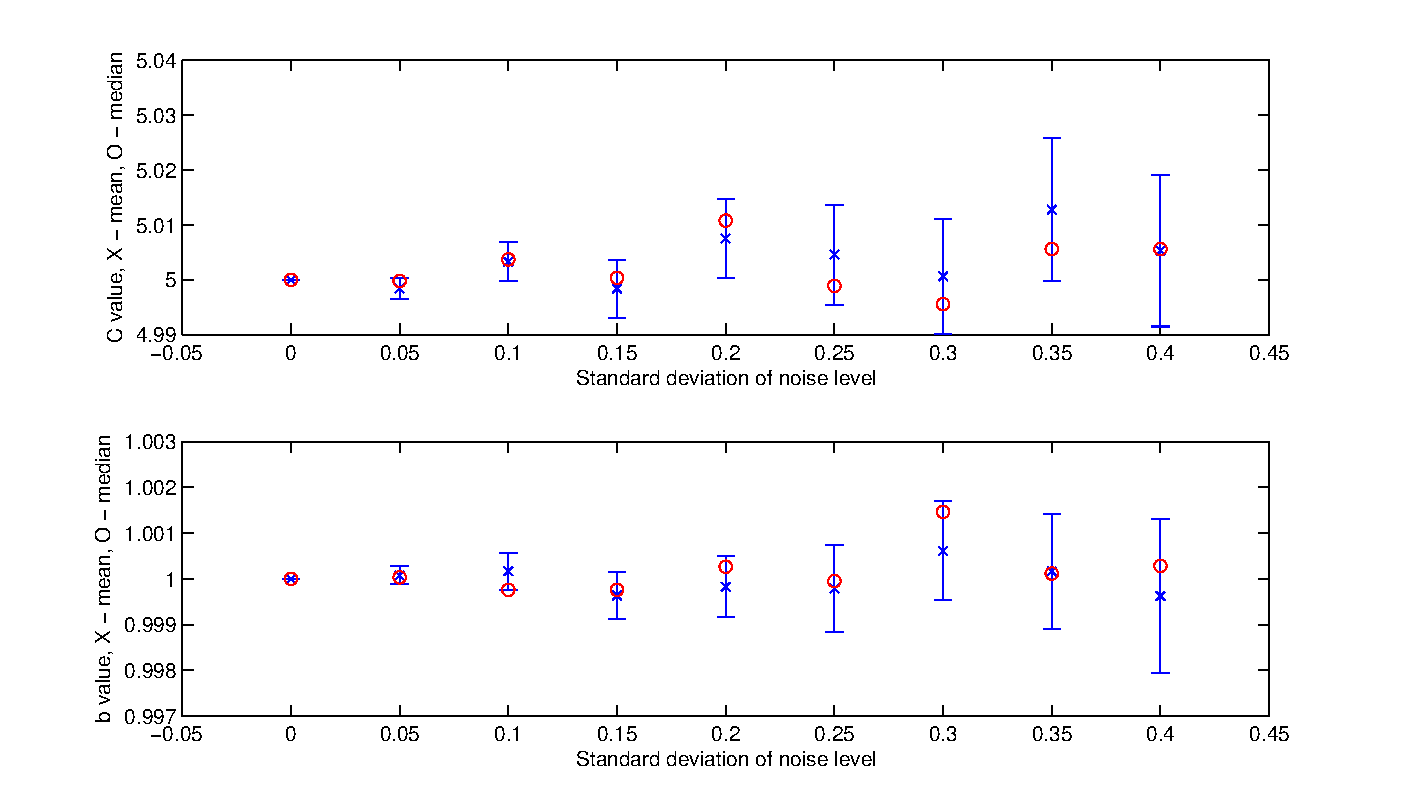
\includegraphics[width=0.6\textwidth]{images/section-3b}
  \caption{Testing the Identification Function\label{3b-fig}}
\end{figure}
